\documentclass{article}


\usepackage{arxiv}
\usepackage{amsmath}
\usepackage{algorithm}
\usepackage[noend]{algpseudocode}

\usepackage{graphicx}

\usepackage[utf8]{inputenc} % allow utf-8 input
\usepackage[T1]{fontenc}    % use 8-bit T1 fonts
\usepackage{hyperref}       % hyperlinks
\usepackage{url}            % simple URL typesetting
\usepackage{booktabs}       % professional-quality tables
\usepackage{amsfonts}       % blackboard math symbols
\usepackage{nicefrac}       % compact symbols for 1/2, etc.
\usepackage{microtype}      % microtypography
\usepackage{lipsum}

\title{A hyperdimensional code for sequences and trees inspired by chromosomal crossover}

\author{
  Rich ~Pang\thanks{https://rkp.science} \\
  Computational Neuroscience Center\\
  Department of Physiology and Biophysics\\
  University of Washington\\
  Seattle, WA 98195-7290 \\
  \texttt{rpang at uw dot edu} \\
}

\begin{document}
\maketitle

\begin{abstract}
I present a method for encoding structured information in fixed-length vectors. Drawing on ideas from high-dimensional (HD) computing, the presented scheme encodes elements of information as HD random vectors and sequences of elements by (pseudo-)randomly weaving these vectors together via an operation analogous to chromosomal crossover. "Crossover" codes retain low Hamming distance to both their elements and the codes for the subsequences used to build them, yet high distance to alternative elements or sequences. Accurate decoding can thus occur via greedy reconstruction of the representation. Unlike most machine-learning approaches, crossover (as in other HD computing schemes) requires no training, making it highly amenable to mathematical analysis. I derive several properties of crossover and discuss its relevance to neuroscience and artificial intelligence.
\end{abstract}


% keywords can be removed
\keywords{Hyperdimensional computing \and Vector symbolic architectures \and Sequence encoding \and Computational neuroscience \and Artificial intelligence \and Cognitive computing}


\section{Introduction}
A common problem in neuroscience and artificial intelligence is how complex events, like spoken sentences, should be represented in a system of relatively fixed dimension. Ideally similar events should have similar representations, and when a new event occurs pre-existing representations shouldn't require substantial rearrangement to prevent confusion.

One approach to solving this has been to assume representations are built from high-dimensional (HD) random vectors \ref{}. Such approach is fundamentally motivated by the observation that independent HD random vectors are very close to orthogonal (and far apart under other distance metrics) with very high probability. Thus, if one considers a codebook where $M$ objects are assigned to $M$ independently sampled HD random vectors, the codes are very unlikely to be confused. 



\section{Problem statement}

Consider a system $X$ of $N$ components $x_1, ..., x_N$, each of which can take any of $Z$ states. That is, $x_j \in G$ where $|G| = Z$. Label the states of $G$ as $1,...,Z$ for conciseness. Let $d(X^A, X^B)$ be the Hamming distance between $X^A$ and $X^B$, scaled to range from 0 and 1, and their similarity $s(X^A, X^B) \equiv 1 - d(X^A, X^B)$.

We wish to establish a decodable mapping from arbitrary objects of cognition to system states, such that objects that are intuitively similar to us map to codes with high similarities. We shall start by considering sequences of symbols then generalize to arbitrary finite nested sets (or equivalently k-ary trees) with symbols as elements (leaves).

\section{Sequence encoding}

\textbf{Summary}

Given a dictionary $D$ of $M$ symbols $s^1, ..., s^M$, we first sample a "C-basis" (crossover basis) $B$ and an auxiliary "mask function" $\mu$ from $P(B)$ and $P(\mu)$, respectively. Using $B$ and $\mu$, we will then deterministically build codes $\{X^Y\}$ of arbitrary sequences $\{Y = (y_1, ..., y_L)\}$, where $y_t \in D$.

\textbf{Setup}

1. Sample a C-basis $B \equiv (X^1, ..., X^M, X^*)$, where each $X^i$ (encoding symbol $s^i$) has components $x^i_j$ sampled uniformly and i.i.d. from $G$, and where $X^*$ is "start" code, also comprised of uniform, i.i.d. components from $G$.

2. Sample a "mask function" $\mu \sim P(\mu)$, where $\mu:(X^A, X^B) \rightarrow [0, 1]^N$ and is represented by a matrix with $N$ rows and $Z^{2N}$ columns, with i.i.d. real-valued elements from $\textrm{Uniform}(0, 1)$. We reference elements of $\mu$ with the notation $\mu(j, X^A, X^B)$. (In practice $\mu$ need not be sampled explicitly, which would take astronomical time; it suffices to use, say, to map $(X^A, X^B)$ using a hash function like SHA-1 to an integer, then sample $N$ times from $\textrm{Uniform}(0, 1)$ from a random number generator seeded with this integer.)

\begin{algorithm}
\caption{Sequence Encoding}

\begin{algorithmic}[0]
\Function{EncodeSequence}{$Y; B, \mu$}
\State $X^Y \gets X^*$
\For{$t \in 1, ..., |Y|$}

\State $mask \gets (\mu(:, X^Y, X^{y_t}) < 1/(t+1)^\gamma)$
\State $X^Y[mask] \gets X^{y_t}[mask]$

\EndFor

\State \textbf{return} $X^Y$
\EndFunction

\end{algorithmic}
\end{algorithm}

 \begin{figure}[!t]
    \centering
    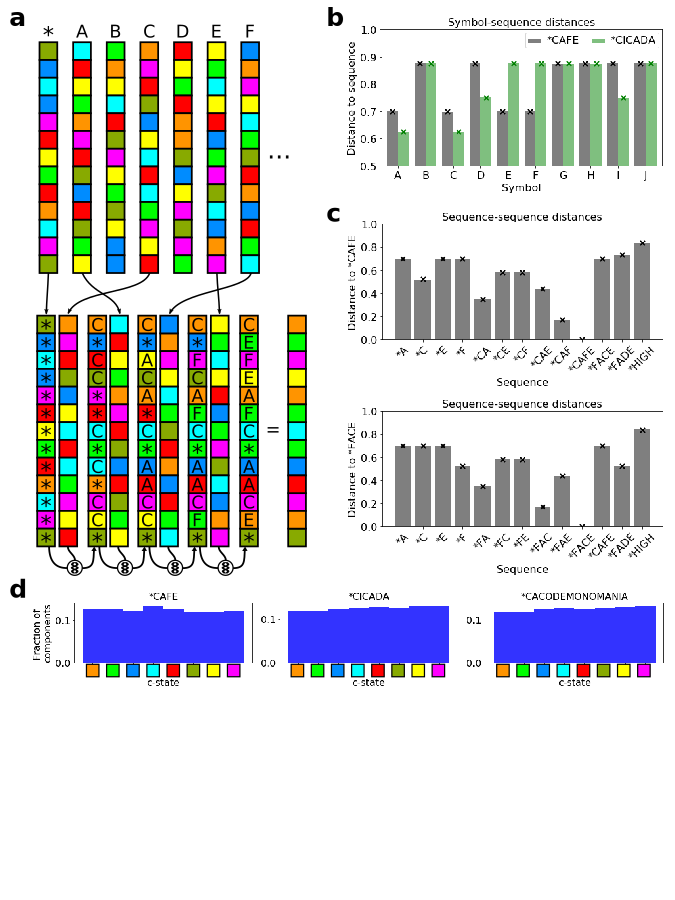
\includegraphics[width=0.8\linewidth]{figs/1_encoding.png}
    \caption{Sequence encoding algorithm and properties.}
 \end{figure}

\section{Properties}

\subsection{Sequence codes have i.i.d. components}
\label{sec:prop-comp-iid}

$$P(X^Y|Y) = \prod\limits_{j=1}^N P(x^Y_j|Y) \quad \textrm{and} \quad P(x^Y_j|Y) = P(x^Y_{j'}|Y) \quad \forall j, j'$$

\subsection{Component distributions are uniform over c-states}
\label{sec:prop-unif-comp-dstr}

$$P(x^Y_j = g|Y) = P(x^Y_j = g'|Y) = \frac{1}{Z} \quad \forall g, g' \in G \quad \textrm{so} \quad P(X^Y|Y) = \prod\limits_{j=1}^N P(x^Y_j|Y) = \frac{1}{Z^N}$$

This implies neither $P(x^Y_j = g|Y)$ nor $P(X^Y|Y)$ are a function of $Y$. Thus, if $Y \sim P(Y)$ we then also have

$$P(x_j) = \sum\limits_Y P(x^Y_j|Y)P(Y) = \frac{1}{Z} \quad \textrm{and} \quad P(X) = \sum\limits_Y P(X^Y|Y)P(Y) = \frac{1}{Z^N}.$$

\subsection{Code statistics are invariant to sequence statistics}

$$P(X^Y|Y) \textrm{ does not depend on any statistic (e.g. length, symbol repetitions, etc) of } Y.$$

\subsection{Sequence information is i.i.d. across components}
\label{sec:prop-info-iid}

Given $B$, $\mu$, and a distribution over sequences $P_Y(Y)$ with entropy $H[Y]$, define the information $I_j | B, \mu$ in component $j$ as the mutual information between $Y$ and $x_j$, i.e.

$$I_j | B, \mu \equiv MI[Y|x_j; B, \mu] = H[Y] - H[Y|x_j; B, \mu] = H[Y] - \sum_g H[Y|x_j = g; B, \mu] P_Y(x_j = g| B, \mu).$$

Then:

$$P(I_1, ..., I_N) = \prod_j P(I_j) \quad \textrm{and} \quad P(I_j) = P(I_{j'}) \quad \forall j, j'.$$

In other words, each component contains independent and equal information about the sequence. (Note that this does not imply $I_j = I_{j'}$ for any given $B$ and $\mu$, since there are $B, \mu$ in which some $x_j$ are less informative about $Y$ than others, e.g. if some $x_j$ by chance has the same c-state for all $Y$.) This means that the code's robustness to random and targeted lesions are equivalent, depending only on how many components were damaged.

\section{Code similarities}

We give results for $\gamma = 1$ here, with results for arbitrary $\gamma$ in the appendix.

Since $x^Y_j$ are i.i.d. across $j$ (\ref{sec:prop-comp-iid}) it follows that $s(X^Y, X^{Y'}) \sim \frac{1}{N}\textrm{Bi}(N, q)$, where $\textrm{Bi}(N, q)$ is a binomial distribution with success probability $q = P(x^Y_j = x^{Y'}_j)$. Thus, $\textrm{E}[s(X^Y, X^{Y'})] = q$ and $\textrm{Var}[s(X^Y, X^{Y'})] = q(1-q)/N$, and it suffices to only compute $q$. For conciseness, we drop the $j$ and write $x \equiv x_j$ from now on. 

\subsection{Similarity between symbol and sequence codes}

If there are $n^i$ repetitions of symbol $i$ appears in $Y$, then:

$$P(x^Y = x^i) = \frac{n^i}{L+1} + \frac{1}{Z}\frac{L+1-n^i}{L+1}$$

which tends to $n^i/(L+1)$ for large $Z$.

\subsection{Similarity between codes for two sequences}

Let $Y = (y_1, ..., y_L)$ and $Y' = (y'_1, .., y'_{L'})$ be two sequences that share a starting subsequence of length $t$. I.e. $y_1 = y'_1, ..., y_t = y'_t$, but either $y_{t+1} \neq y'_{t+1}$, $t = L$, or $t = L'$. We write that $Y_{1:t} = Y'_{1:t}$, and we refer to the second parts of the sequences as $Y_{t+1:L}$ and $Y'_{t+1:L'}$, respectively. We must deal specially with starting subsequences because sequence codes are constructed from beginning to end.

Let $\mathbf{n}_u$ be the length-$M$ symbol count vector for $Y_{1:t} = Y'_{1:t}$ with $\mathbf{1}^T\mathbf{n}_u = t$. Let $\mathbf{n}_v$ and $\mathbf{n}_{v'}$ be the symbol count vectors for $Y_{t+1:L}$ and $Y'_{t+1:L'}$, respectively, with $\mathbf{1}^T\mathbf{n}_{v} = L - t$ and $\mathbf{1}^T\mathbf{n}_{v'} = L' - t$. Then:

$$P(x^Y = x^{Y'}) = \frac{t+1}{L+1}\frac{t+1}{L'+1}$$

$$+ \frac{1}{L+1}\frac{1}{L'+1}\left[\mathbf{n}^T_v\mathbf{n}_{v'} + \left((L-t)(L'-t) - \mathbf{n}^T_v\mathbf{n}_{v'} \right)\frac{1}{Z}\right]
$$

$$+\frac{1}{L+1}\frac{1}{L'+1}\left[
\mathbf{n}^T_{u}\mathbf{n}_{v'} + \left((t+1)(L'-t) - \mathbf{n}^T_{u}\mathbf{n}_{v'} \right)\frac{1}{Z}
\right]
$$

$$+\frac{1}{L+1}\frac{1}{L'+1}\left[
\mathbf{n}^T_{v}\mathbf{n}_{u} + \left((L-t)(t+1) - \mathbf{n}^T_{v}\mathbf{n}_{u} \right)\frac{1}{Z}
\right]
$$

This means that when $Y'$ is a starting subsequence of $Y$, i.e. $Y' = Y_{1:t}$ then the two sequences' expected similarity is

$$P(x^{Y'} = x^Y) = \frac{1}{(L+1)(t+1)}\left((t+1)^2 + \frac{Z-1}{Z}\mathbf{n}^T_{1:t}\mathbf{n}_{t+1:L} + \frac{(t+1)(L-t)}{Z}\right).$$

\section{Sequence decoding}
How to decode a sequence

\begin{algorithm}
\caption{Sequence Decoding}

\begin{algorithmic}[0]
\Function{DecodeSequence}{$X^Y; B, \mu$}
\State $\hat{X}^Y \gets X^*$
\State $d \gets \textrm{Hamming}(\hat{X}^Y , X^*)$
\State $t = 1$

\While{$d > 0$}

\State $(i_{best}, \hat{X}^Y_{best}, d_{best}) \gets (Null, Null, 1)$

    \For{$i_{temp} \in 1, ..., M$}
    
        \State $\hat{X}^Y_{temp} \gets \hat{X}^Y $
        \State $ mask \gets (\mu(:, \hat{X}^Y_{temp}, X^{i_{temp}}) < 1/(t+1)^\gamma)$
        \State $\hat{X}^Y_{temp}[mask] \gets X^{i_{temp}}[mask]$
        \State $d_{temp} \gets \textrm{Hamming}(X^Y, \hat{X}^Y_{temp})$
        
        \If{$d_{temp} < d_{best}$}
            
            \State $(i_{best}, \hat{X}^Y_{best}, d_{best}) \gets (i_{temp}, \hat{X}^Y_{temp}, d_{temp})$
            
        \EndIf
    \EndFor
    
    \If{$d_{best}\geq d$}
    
        \State \textbf{return} $y_1, ..., y_t$
        
    \Else
    
        \State $(y_t, \hat{X}^Y, d) \gets (i_{best}, \hat{X}^Y_{best}, d_{best})$
        \State $t = t+1$
        
    \EndIf

\EndWhile

\State \textbf{return} $y_1, ..., y_t$
\EndFunction

\end{algorithmic}
\end{algorithm}

\begin{figure}[!t]
    \centering
    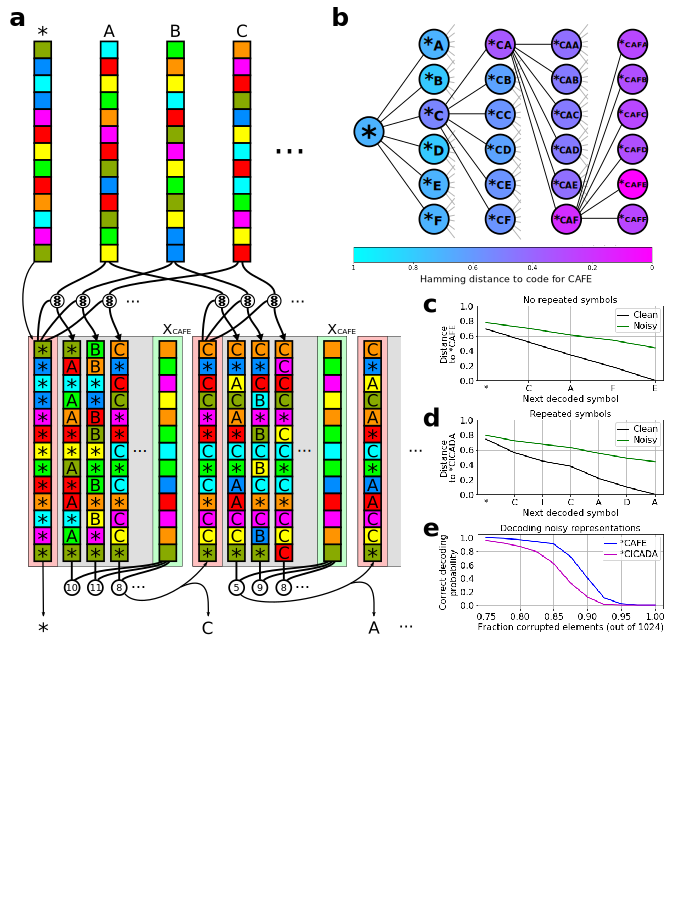
\includegraphics[width=0.8\linewidth]{figs/2_decoding.png}
    \caption{Sequence decoding algorithm and properties.}
 \end{figure}

\section{Improving decoding with $\gamma$}

\begin{figure}[!t]
    \centering
    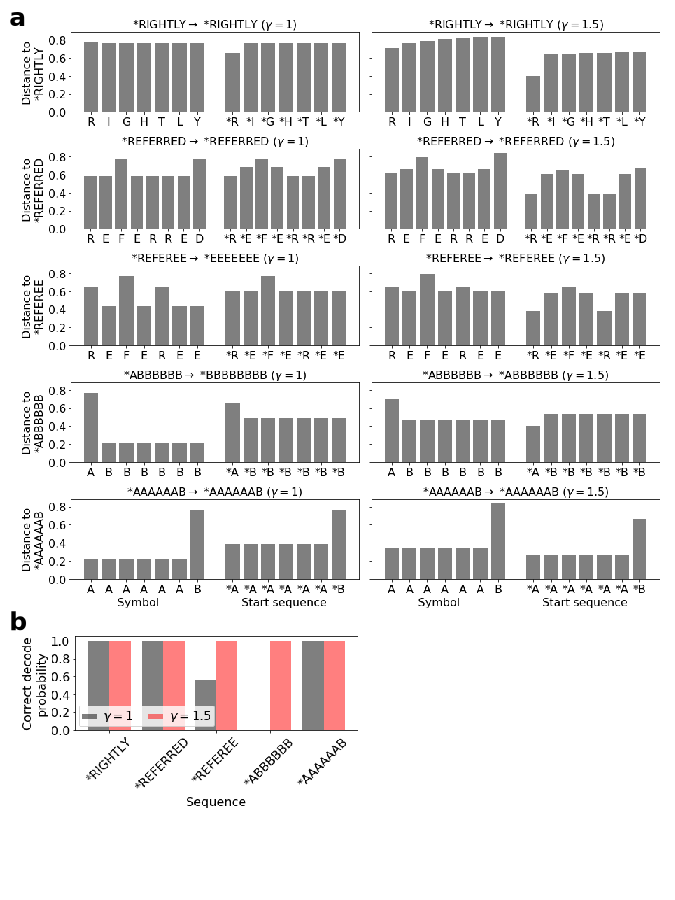
\includegraphics[width=0.8\linewidth]{figs/3_gamma.png}
    \caption{Dependence of sequence codes on $\gamma$.}
 \end{figure}

\section{Trees}

\begin{algorithm}
\caption{Tree Encoding}

\begin{algorithmic}[0]
\Function{EncodeTree}{$T; B, \mu$}

\State $D^T \gets \{i: X^i \textrm{ \textbf{for} } i \in 1, ..., M\}$

\For{$J \in T$}

    \State $X^T \gets D^T[J^1]$
    \For{$k \in 2, ..., |J|$}
        \State $mask \gets (k/|J| \leq \mu(:, J) \leq (k+1)/|J|)$
        \State $X^T[mask] \gets D^T[J^k][mask]$
    \EndFor
    
    \State $D^T[J] \gets X^T$
\EndFor

\State \textbf{return} $D^T[T[\textrm{end}]]$
\EndFunction

\end{algorithmic}
\end{algorithm}

\begin{figure}[!t]
    \centering
    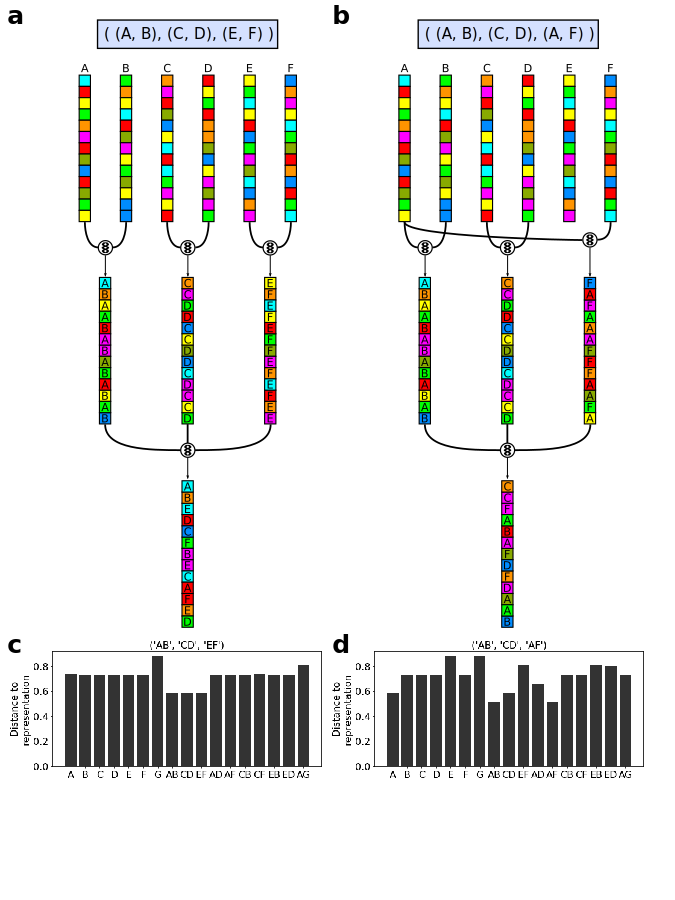
\includegraphics[width=0.8\linewidth]{figs/4_trees.png}
    \caption{Tree encoding algorithm and properties.}
 \end{figure}

\begin{algorithm}
\caption{Tree Decoding}

\begin{algorithmic}[0]
\Function{DecodeTree}{$X^T; B, \mu$}
\State $D^T \gets \{i: X^i \textrm{ \textbf{if} } \textrm{Hamming}(X^T, X^i) < d_{exclude} \textrm{ \textbf{for} } i \in 1, ..., M\}$
\State $T \gets ()$

\State $d \gets 1$
    
\While{$d > 0$}

    \State $(J_{best}, \hat{X}^T_{best}, d_{best}) \gets (Null, Null, 1)$
    
    \For{$J_{temp} \in \{J\}$}
        
        \State $\hat{X}^T_{temp} \gets D^T[J^1]$
        \For{$k \in 2, ..., |J_{temp}|$}
            \State $mask \gets k/|J_{temp}| \leq \mu(:, J_{temp}) \leq (k+1)/|J_{temp}|$
            \State $\hat{X}^T_{temp}[mask] \gets D^T[J^k_{temp}][mask]$
        \EndFor
        
        \State $d_{temp} \gets \textrm{Hamming}(X^T, \hat{X}^T_{temp})$
        
        \If{$d_{temp} < d_{best}$}
            \State $(J_{best}, \hat{X}^T_{best}, d_{best}) \gets (J_{temp}, \hat{X}^T_{temp}, d_{temp})$
        \EndIf
    \EndFor
    
    \If{$d_{best} \geq d$}
        \State \textbf{return} $T[\textrm{end}]$
        
    \Else
        \State $(D^T[J_{best}], d) \gets (\hat{X}^T_{best}, d_{best})$
        \State $\textrm{Append}(T, J_{best})$
    \EndIf

\EndWhile

\State \textbf{return} $T[\textrm{end}]$
\EndFunction

\end{algorithmic}
\end{algorithm}

\section{Mask correlations}

\begin{figure}[!t]
    \centering
    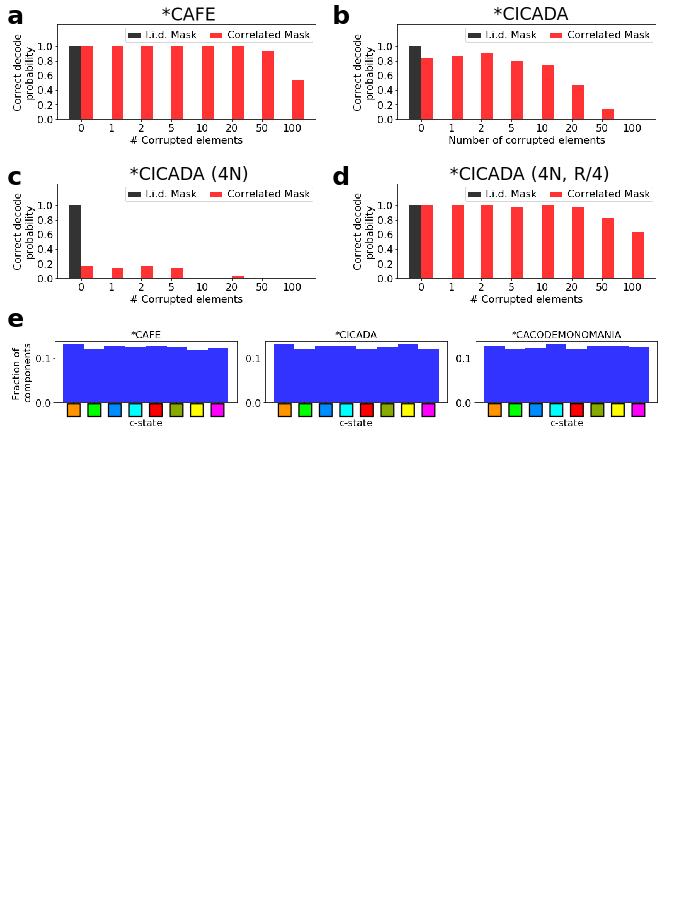
\includegraphics[width=0.8\linewidth]{figs/5_mask_corrs.png}
    \caption{Robustness to encoding noise through mask correlations.}
 \end{figure}

\section{Discussion}




\bibliographystyle{unsrt}  
%\bibliography{references}  %%% Remove comment to use the external .bib file (using bibtex).
%%% and comment out the ``thebibliography'' section.


%%% Comment out this section when you \bibliography{references} is enabled.
\begin{thebibliography}{1}

\bibitem{kour2014real}
George Kour and Raid Saabne.
\newblock Real-time segmentation of on-line handwritten arabic script.
\newblock In {\em Frontiers in Handwriting Recognition (ICFHR), 2014 14th
  International Conference on}, pages 417--422. IEEE, 2014.

\bibitem{kour2014fast}
George Kour and Raid Saabne.
\newblock Fast classification of handwritten on-line arabic characters.
\newblock In {\em Soft Computing and Pattern Recognition (SoCPaR), 2014 6th
  International Conference of}, pages 312--318. IEEE, 2014.

\bibitem{hadash2018estimate}
Guy Hadash, Einat Kermany, Boaz Carmeli, Ofer Lavi, George Kour, and Alon
  Jacovi.
\newblock Estimate and replace: A novel approach to integrating deep neural
  networks with existing applications.
\newblock {\em arXiv preprint arXiv:1804.09028}, 2018.

\end{thebibliography}

\section{Appendix}

\subsection{Proof: Sequence codes have i.i.d. components}

Denoting $Y_{1:t} \equiv (y_1, ..., y_t)$ with $Y_{1:L} = Y$, and $B_j \equiv (x^1_j, ..., x^M_j, x^*_j)$, we want to show that $x_j^{Y_{1:t}}$ are independent across $j$ for all $t$.

We will frequently use the fact that if $A_1, ..., A_N$ are independent, then so are $f(A_1), ..., f(A_N)$. In particular, we note that $x_j^{Y_{1:t}}$ is a strict function of $\xi^t_j \equiv \{x_j^{Y_{1:t-1}}, ..., x_j^{Y_{1:0}}, B_j, \mu(j, X^*, X^{y_1}), \mu(j, X^{Y_{1:1}}, X^{y_2}), ..., \mu(j, X^{Y_{1:t-1}}, X^{y_t})\}.$ Therefore if $\xi^t_j$ are independent across $j$, so are $x_j^{Y_{1:t}}$. Thus, it suffices to show $\xi^t_j$ are independent across $j$ for all $t$.

We proceed by induction:

\textbf{Base case:} $\xi^1_j = \{x^{Y_{1:0}}_j, B_j, \mu(j, X^{Y_{1:0}}, X^{y_1})\} = \{x^*_j, B_j, \mu(j, X^*, X^{y_1})\}$, which are all i.i.d., so $\xi^1_j$ are independent across $j$.

\textbf{Inductive step:} If $\xi^t_j$ are independent across $j$ then so are $\{x_j^{Y_{1:t}}\} \cup \xi^t_j$, since this is just a function of $\xi^t_j$. Further, $\{x_j^{Y_{1:t}}\} \cup \xi^t_j \cup \{\mu(j, X^{Y_{1:t}}, X^{y_{t+1}})\}$ must also be independent across $j$. To see this, consider the following two cases.

First, most likely is that $\mu(j, X^{Y_{1:t}}, X^{y_{t+1}})$ has never been used in the construction of $X^{Y_{1:t-1}}$, so it is independent from $\{x_j^{Y_{1:t}}\} \cup \xi^t_j$ while also independent across $j$. Therefore, their union is independent across $j$.

In the second, less likely case, $\mu(j, X^{Y_{1:t}}, X^{y_{t+1}})$ \textit{was} used to construct $X^{Y_{1:t-1}}$ at some point in the past, i.e. $(X^{Y_{1:t}}, X^{y_{t+1}}) = (X^{Y_{1:t'}}, X^{y_{t'+1}})$ for some $t' < t$. In this case, however, the term $\mu(j, X^{Y_{1:t}}, X^{y_{t+1}}) = \mu(j, X^{Y_{1:t'}}, X^{y_{t'+1}})$ is already included in $\xi^t_j$, and so the independence across $j$ is not affected because no new random variables are added. Thus, $\{x_j^{Y_{1:t}}\} \cup \xi^t_j \cup \{\mu(j, X^{Y_{1:t}}, X^{y_{t+1}})\}$ is independent across $j$.

Since $\{x_j^{Y_{1:t}}\} \cup \xi^t_j \cup \{\mu(j, X^{Y_{1:t}}, X^{y_{t+1}})\} = \xi^{t+1}_j$, we have that $\xi^t_j$ being independent across $j$ implies that $\xi^{t+1}_j$ is independent across $j$, completing the inductive step.

Therefore $x_j^{Y_{1:t}}$ is independent across $j$ for all $t$, in other words $P(X^Y|Y) = \prod\limits_{j=1}^N P(x^Y_j|Y)$.

The equality $P(x^Y_j|Y) = P(x^Y_{j'}|Y) \quad \forall j, j'$ arises because no component is treated differently from any other in our algorithm, so symmetry implies they can have no statistical differences.

\subsection{Proof: Component distributions are uniform over c-states}

$P(x^Y_j = g|Y) = P(x^Y_j = g'|Y)$ for $g \neq g'$ arises because all $g$ in our model are treated identically, so symmetry implies any functions of them can have no statistical differences. Since these must add to $1$ when summed over $g \in G$, and $|G| = Z$, we must also have $P(x^Y_j = g|Y) = 1/Z.$

\subsection{Proof: Code statistics are invariant to sequence statistics}

This follows from \ref{sec:prop-unif-comp-dstr}, since $P(x^Y_j|Y) = 1/Z$. Therefore the statistics of crossover codes do not depend on any aspect about the sequence being encoded. This distinguishes crossover, for instance, from representations that grow more or less crowded with the complexity of the sequence they represent.

\subsection{Proof: Sequence information is i.i.d. across components}

Since the components for one sequence $Y$ are i.i.d. (\ref{sec:prop-comp-iid}) Therefore, while the $x^Y_j$ and $x^{Y'}_j$ might be dependent (e.g. if $Y$ and $Y'$ are very similar; see below), there can be no dependencies between $x^Y_j$ and $x^{Y'}_{j'}$ for $j \neq j'$. Therefore $\{x^{Y_1}_j, ..., x^{Y_{N_Y}}_j\}$ is independent across $j$. Since $I_j$ is a function of $\{x^{Y_1}_j, ..., x^{Y_{N_Y}}_j\}$, $I_j$ is independent across $j$ also. Since no $j$ is treated specially in our algorithm, $I_j$ must also be identically distributed, so given $P(Y)$, $I_j$ is i.i.d.

\subsection{Code similarity derivations}

Since $x^Y_j$ are i.i.d. across $j$ (\ref{sec:prop-comp-iid}) it follows that $s(X^Y, X^{Y'}) \sim \frac{1}{N}\textrm{Bi}(N, q)$, where $\textrm{Bi}(N, q)$ is a binomial distribution with success probability $q = P(x^Y_j = x^{Y'}_j)$. Thus, $\textrm{E}[s(X^Y, X^{Y'})] = q$ and $\textrm{Var}[s(X^Y, X^{Y'})] = q(1-q)/N$, and it suffices to only compute $q$. For conciseness, we drop the $j$ and write $x \equiv x_j$ from now on.

We define and compute a few useful quantities that will keep our calculations more precise.

1. $P(x^Y \leftarrow y_t)$ is the probability that $x^Y$ was taken from the $t$-th element of $Y$, that is, $1/(t+1)^\gamma$ times the probability it was not overwritten between $t+1$ and $L$ (including occasions where it was overwritten by the same state). For notational convenience we call this $f^{\gamma,L}_t$. We then have:

$$f^{\gamma,L}_t \equiv P(x^Y \leftarrow y_t) = \frac{1}{(t+1)^\gamma}\prod\limits_{t' = t+1}^L\left(1 - \frac{1}{(t'+1)^\gamma}\right).$$

Note that this is not a function of $x^Y$. Also note that $f^{1,L}_t = 1/(L+1)$, which is not a function of $t$.

2. $P(x^Y \leftarrow i)$ is the probability that $x^Y$ was taken from symbol $i$, which will depend on how many times $i$ was present in $Y$. We compute this by summing the probabilities of all ways this could have occurred.

Suppose $y_t = i$ for $t_1 < ... < t_{n^i}$, with $\sum_i n^i = L$. We can divide the combinatorial ways $x^Y$ could have ended up being taken from $i$ into $n^i$ cases. First, $x^Y$ could have been taken from $y_{t_1}$ then never overwritten, whose probability is $f^{\gamma,L}_{t_1}$. Next, it could have been taken from $y_{t_2}$ then never overwritten (regardless of whether it was taken from $y_{t_1}$), whose probability is $f^{\gamma,L}_{t_2}$. And so forth until $t_{n^i}$. Note that these $n^i$ cases are mutually non-overlapping and cover all possible ways that $x^Y$ could have been taken from $i$. Thus

$$P(x^Y \leftarrow i) = f^{\gamma,L}_{t_1} + ... + f^{\gamma,L}_{t_{n^i}}$$.

When $\gamma = 1$, $P(x^Y \leftarrow i) = n/(L+1)$.

3. $P(x^Y \leftarrow Y_{1:t})$ is the probability that $x^Y$ was not overwritten from $t+1$ to $L$. This is just

$$P(x^Y \leftarrow Y_{1:t}) = \prod\limits_{t' = t+1}^L \left(1 - \frac{1}{(t'+1)^\gamma}\right) = (t+1)^\gamma f^{\gamma,L}_t.$$

When $\gamma = 1$, $P(x^Y \leftarrow Y_{1:t}) = (t+1)/(L+1)$.

4. $P(x^Y \leftarrow i|x^Y \not \leftarrow Y_{1:t})$ is the probability that $x^Y$ came from $i$ given that it did not come from $Y_{1:t}$ (i.e. given that it was overwritten at some point from $t+1$ to $L$). Suppose $y_s = i$ for $t < s_1 < ... < s_{n^i_v}$ where $n^i_v$ is the number of times symbol $i$ appears in $Y_{t+1:L} \equiv (y_{t+1}, ..., y_L)$, with $\sum\limits_i n^i_v = L-t$.

We compute $P(x^Y \leftarrow i|x^Y \not \leftarrow Y_{1:t})$ by summing over the probabilities of all the ways this could have occurred. Similar to the calculation for $P(x^Y \leftarrow i)$, we have

$$P(x^Y \leftarrow i|x^Y \not \leftarrow Y_{1:t}) = P(x^Y \leftarrow y_{s_1}| x^Y \not \leftarrow Y_{1:t}) + ... + P(x^Y \leftarrow y_{s_{n^i_v}}| x^Y \not \leftarrow Y_{1:t}).$$

By Bayes' Rule:

$$P(x^Y \leftarrow y_{s_k}| x^Y \not \leftarrow Y_{1:t}) = \frac{P(x^Y \not \leftarrow Y_{1:t}| x^Y \leftarrow y_{s_k})P(x^Y \leftarrow y_{s_k})}{P(x^Y \not\leftarrow Y_{1:t})} = \frac{P(x^Y \leftarrow y_{s_k})}{P(x^Y \not\leftarrow Y_{1:t})}$$

since if $x^Y$ came from $y_{s_k}$, which is in the part of $Y$ after $t$, then $x^Y$ could have not have come from $Y_{1:t}$. We have already computed the numerator and denominator (which is just $1 - P(x^Y \leftarrow Y_{1:t}))$, so

$$P(x^Y \leftarrow i|x^Y \not \leftarrow Y_{1:t}) = \frac{1}{P(x^Y \not\leftarrow Y_{1:t})}\left( f^{\gamma,L}_{s_1} + ... + f^{\gamma,L}_{s_{n^i_v}} \right).$$

When $\gamma = 1$ this reduces to $P(x^Y \leftarrow i|x^Y \not \leftarrow Y_{1:t}) = \frac{n^i_v}{L-t}$, i.e. it is proportional to how many times $i$ appears in the second part of the sequence $Y_{t+1:L}$.

We now calculate how similar a sequence code is to any symbol code, as well as to other sequence codes.

\subsubsection{Derivation: Similarity between symbol and sequence codes}

$$P(x^Y = x^i) = P(x^Y \leftarrow i)P(x^Y = x^i|x^Y \leftarrow i) + P(x^Y \not \leftarrow i)P(x^Y = x^i|x^Y \not \leftarrow i)
= P(x^Y \leftarrow i) + P(x^Y \not \leftarrow i)\frac{1}{Z}$$

$$= \sum\limits_{t \in (t_1, ..., t_{n^i})}f^{\gamma,L}_t + \left(1 - \sum\limits_{t \in (t_1, ..., t_{n^i})}f^{\gamma,L}_t\right)\frac{1}{Z}
= \sum\limits_{t \in (t_1, ..., t_{n^i})}\left(1 - \frac{1}{Z}\right)f^{\gamma,L}_t + \frac{1}{Z}$$

\subsubsection{Derivation: Similarity between codes for two sequences}

Let $u^i$ index the times $i$ appears in $Y_{1:t}$, $v^i$ the times $i$ appears in $Y_{t+1:L}$, and $(v')^i$ the times $i$ appears in $Y'_{t+1:L'}$. Let $n^i_u$ count how many times $i$ appears in $Y_{1:t}$, $n^i_v$ the number of times $i$ appears in $Y_{t+1:L}$, and $n^i_{v'}$ the number of times $i$ appears in $Y'_{t+1:L'}$. We also write these in vector format as $\mathbf{n}_u$, $\mathbf{n}_v$, and $\mathbf{n}_{v'}$, respectively.

Since $Y_{1:t} = Y'_{1:t}$,  first note that $X^{Y_{1:t}} = X^{Y'_{1:t}}$, so $x^{Y_{1:t}} = x^{Y'_{1:t}}$. We wish to find $P(x^Y = x^{Y'})$.

The event $x^Y = x^{Y'}$ can occur in 4 distinct ways, whose probabilities sum to $P(x^Y = x^{Y'})$. At present we assume a negligible chance two sequence or symbol codes are exactly identical.

\textbf{Case 1}: $(x^Y \leftarrow Y_{1:t}) \land (x^{Y'} \leftarrow Y'_{1:t})$, i.e. neither $x$ is overwritten at $t+1$ or later. These events are independent, so

$$P(\textrm{Case 1}) = P(x^Y \leftarrow Y_{1:t})P(x^{Y'} \leftarrow Y'_{1:t}) = (t+1)^\gamma f^{\gamma,L}_t(t+1)^\gamma f^{\gamma,L'}_t$$

When $\gamma = 1$, then:

$$P(\textrm{Case 1}) = \frac{t+1}{L+1}\frac{t+1}{L'+1}$$.

\textbf{Case 2}: $(x^Y \not\leftarrow Y_{1:t}) \land (x^{Y'} \not\leftarrow Y'_{1:t}) \land (x^Y = x^{Y'})$, i.e. $x$ is overwritten in both sequences at some point between $t+1$ and $L$ or $L'$, but by the same c-state. Since the first two conditions are again independent we have

$$P(\textrm{Case 2}) = P(x^Y \not\leftarrow Y_{1:t})P(x^{Y'} \not\leftarrow Y'_{1:t})P(x^Y = x^{Y'}|x^Y, x^{Y'} \not\leftarrow Y_{1:t})$$

$$= [1 - (t+1)^\gamma f^{\gamma,L}_t][1 - (t+1)^\gamma f^{\gamma,L'}_t]P(x^Y = x^{Y'}|x^Y, x^{Y'} \not\leftarrow Y_{1:t})$$

where we recall that $Y_{1:t} = Y'_{1:t}$. When $\gamma = 1$ this simplifies to

$$P(\textrm{Case 2}) = \frac{L-t}{L+1}\frac{L'-t}{L'+1}P(x^Y = x^{Y'}|x^Y, x^{Y'} \not\leftarrow Y_{1:t})$$

To find $P(x^Y = x^{Y'}|x^Y, x^{Y'} \not\leftarrow Y_{1:t})$ we note that if both $x$'s are overwritten, they can end up with the same c-state if (1) $x^Y$ and $x^{Y'}$ are taken from the same symbol $i$, whose probability we write as $P(x^Y, x^{Y'} \leftarrow same|x^Y, x^{Y'} \not\leftarrow Y_{1:t})$ or (2) $x^Y$ and $x^{Y'}$ are taken from different symbol codes but end up with the same c-state. That is,

$$P(x^Y = x^{Y'}|x^Y, x^{Y'} \not\leftarrow X^{Y_{1:t}}) =$$

$$P(x^Y, x^{Y'} \leftarrow same|x^Y, x^{Y'} \not\leftarrow X^{Y_{1:t}}) + [1 - P(x^Y, x^{Y'} \leftarrow same|x^Y, x^{Y'} \not\leftarrow Y_{1:t})]\frac{1}{Z}.$$

$P(x^Y, x^{Y'} \leftarrow same|x^Y, x^{Y'} \not\leftarrow X^{Y_{1:t}})$ is the sum over $i \in \{1, ..., M\}$ of the probabilities that both $x^Y$ and $x^{Y'}$ ended up being taken from $i$. These events are independent, so:

$$P(x^Y, x^{Y'} \leftarrow i|x^Y, x^{Y'} \not\leftarrow X^{Y_{1:t}}) = P(x^Y \leftarrow i|x^Y, x^{Y'} \not\leftarrow X^{Y_{1:t}})P(x^{Y'} \leftarrow i|x^Y, x^{Y'} \not\leftarrow X^{Y_{1:t}})$$

$$ = \frac{\sum\limits_{v^i} f_{v^i}^{\gamma,L}}{1 - (t+1)^\gamma f^{\gamma,L}_t} \frac{\sum\limits_{(v')^i} f^{\gamma,L'}_{(v')^i}}{1 - (t+1)^\gamma f^{\gamma,L'}_t}.$$

When $\gamma = 1$, this simplifies to

$$\frac{n^i_v}{L-t}\frac{n^i_{v'}}{L'-t}$$.

Thus

$$P(x^Y, x^{Y'} \leftarrow same|x^Y, x^{Y'} \not\leftarrow X^{Y_{1:t}}) = \sum_i \frac{\sum\limits_{v^i} f^{\gamma,L}_{v^i}}{1 - (t+1)^\gamma f^{\gamma,L}_t} \frac{\sum\limits_{(v')^i} f^{\gamma,L'}_{(v')^i}}{1 - (t+1)^\gamma f^{\gamma,L'}_t}.$$

When $\gamma = 1$ this is

$$P(x^Y, x^{Y'} \leftarrow same|x^Y, x^{Y'} \not\leftarrow X^{Y_{1:t}}) = \sum_i \frac{n^i_vn^i_{v'}}{(L-t)(L'-t)} = \frac{\mathbf{n}^T_v\mathbf{n}_{v'}}{(L-t)(L'-t)}$$

i.e. when $\gamma = 1$ the probability that $x^Y$ came from the same symbol, given that it was overwritten in the second part of both sequence constructions, is just the normalized dot product of the symbol-count vectors for the second parts of the two sequences.

Thus

$$P(x^Y = x^{Y'}|x^Y, x^{Y'} \not\leftarrow X^{Y_{1:t}}) = $$

$$\sum_i \frac{\sum\limits_{v^i} f^{\gamma,L}_{v^i}}{1 - (t+1)^\gamma f^{\gamma,L}_t} \frac{\sum\limits_{(v')^i} f^{\gamma,L'}_{(v')^i}}{1 - (t+1)^\gamma f^{\gamma,L'}_t} + \left(1 - \sum_i \frac{\sum\limits_{v^i} f^{\gamma,L}_{v^i}}{1 - (t+1)^\gamma f^{\gamma,L}_t} \frac{\sum\limits_{(v')^i} f^{\gamma,L'}_{(v')^i}}{1 - (t+1)^\gamma f^{\gamma,L'}_t}\right)\frac{1}{Z}$$

When $\gamma = 1$

$$P(x^Y = x^{Y'}|x^Y, x^{Y'} \not\leftarrow X^{Y_{1:t}}) = \frac{\mathbf{n}^T_v\mathbf{n}_{v'}}{(L-t)(L'-t)} + \left(1 - \frac{\mathbf{n}^T_v\mathbf{n}_{v'}}{(L-t)(L'-t)} \right)\frac{1}{Z}.$$

Thus

$$P(\textrm{Case 2}) = [1 - (t+1)^\gamma f^{\gamma,L}_t][1 - (t+1)^\gamma f^{\gamma,L'}_t] \times$$

$$\left[
\sum_i \frac{\sum\limits_{v^i} f^{\gamma,L}_{v^i}}{1 - (t+1)^\gamma f^{\gamma,L}_t} \frac{\sum\limits_{(v')^i} f^{\gamma,L'}_{(v')^i}}{1 - (t+1)^\gamma f^{\gamma,L'}_t} + \left(1 - \sum_i \frac{\sum\limits_{v^i} f^{\gamma,L}_{v^i}}{1 - (t+1)^\gamma f^{\gamma,L}_t} \frac{\sum\limits_{(v')^i} f^{\gamma,L'}_{(v')^i}}{1 - (t+1)^\gamma f^{\gamma,L'}_t}\right)\frac{1}{Z}
\right]$$

When $\gamma = 1$:

$$P(\textrm{Case 2}) = \frac{L-t}{L+1}\frac{L'-t}{L'+1}\left[\frac{\mathbf{n}^T_v\mathbf{n}_{v'}}{(L-t)(L'-t)} + \left(1 - \frac{\mathbf{n}^T_v\mathbf{n}_{v'}}{(L-t)(L'-t)} \right)\frac{1}{Z}\right].$$

\textbf{Case 3}: $(x^Y \leftarrow Y_{1:t}) \land (x^{Y'} \not\leftarrow Y'_{1:t}) \land (x^Y = x^{Y'})$, i.e. $x$ is untouched in the first sequence but overwritten in the second, but happens to be overwritten by $x^{Y_{1:t}}$. Once again the first two events are independent, so 

$$P(\textrm{Case 3}) = (t+1)^\gamma f^{\gamma,L}_t[1-(t+1)^\gamma f^{\gamma,L'}_t]P(x^Y = x^{Y'}|x^Y \leftarrow Y_{1:t}, x^{Y'} \not\leftarrow Y'_{1:t}).$$

When $\gamma = 1$:

$$P(\textrm{Case 3}) = \frac{t+1}{L+1}\frac{L'-t}{L'+1}P(x^Y = x^{Y'}|x^Y \leftarrow Y_{1:t}, x^{Y'} \not\leftarrow Y'_{1:t}).$$

By similar reasoning as in Case 2, the event $(x^Y = x^{Y'}|x^Y \leftarrow X^{Y_{1:t}}, x^{Y'} \not\leftarrow X^{Y'_{1:t}})$ can occur if (1) $x^Y$ and $x^{Y'}$ are taken from the same symbol $i$ or (2) $x^Y$ and $x^{Y'}$ are taken from different symbols but end up with the same c-state.

Following similar logic as in Case 2, except swapping $Y^{t+1:L}$ with $Y^{1:t}$ we thus have

$$P(x^Y = x^{Y'}|x^Y \leftarrow Y_{1:t}, x^{Y'} \not\leftarrow Y'_{1:t}) =$$

$$\left[
\sum_i \frac{\sum\limits_{u^i} f_{u^i}^{\gamma, t} \sum\limits_{(v')^i} f_{(v')^i}^{\gamma,L'}}{1 - (t+1)^\gamma f^{\gamma,L'}_t} 
+ \left(1 - \sum_i \frac{\sum\limits_{u^i} f_{u^i}^{\gamma, t} \sum\limits_{(v')^i} f_{(v')^i}^{\gamma,L'}}{1 - (t+1)^\gamma f^{\gamma,L'}_t}\right)\frac{1}{Z}
\right]$$

When $\gamma = 1$:

$$P(x^Y = x^{Y'}|x^Y \leftarrow Y_{1:t}, x^{Y'} \not\leftarrow Y'_{1:t}) =
\frac{\mathbf{n}^T_{u}\mathbf{n}_{v'}}{(t+1)(L'-t)} + \left(1 - \frac{\mathbf{n}^T_{u}\mathbf{n}_{v'}}{(t+1)(L'-t)} \right)\frac{1}{Z}$$

Thus,

$$P(\textrm{Case 3}) = (t+1)^\gamma f^{\gamma,L}_t[1-(t+1)^\gamma f^{\gamma,L'}_t] \times 
\left[
\sum_i \frac{\sum\limits_{u^i} f_{u^i}^{\gamma, t} \sum\limits_{(v')^i} f_{(v')^i}^{\gamma,L'}}{1 - (t+1)^\gamma f^{\gamma,L'}_t} 
+ \left(1 - \sum_i \frac{\sum\limits_{u^i} f_{u^i}^{\gamma, t} \sum\limits_{(v')^i} f_{(v')^i}^{\gamma,L'}}{1 - (t+1)^\gamma f^{\gamma,L'}_t}\right)\frac{1}{Z}
\right]$$

And when $\gamma = 1$:

$$P(\textrm{Case 3}) = \frac{t+1}{L+1}\frac{L'-t}{L'+1}\left[
\frac{\mathbf{n}^T_{u}\mathbf{n}_{v'}}{(t+1)(L'-t)} + \left(1 - \frac{\mathbf{n}^T_{u}\mathbf{n}_{v'}}{(t+1)(L'-t)} \right)\frac{1}{Z}
\right].$$

\textbf{Case 4}: $(x^Y \not \leftarrow Y_{1:t}) \land (x^{Y'} \leftarrow Y'_{1:t}) \land (x^Y = x^{Y'})$, i.e. $x$ is untouched in the second sequence but overwritten in the first, but happens to be overwritten by $x^{Y'_{1:t}}$. This is symmetric to Case 3, so

$$P(\textrm{Case 4}) = [1 - (t+1)^\gamma f^{\gamma,L}_t](t+1)^\gamma f^{\gamma,L'}_t \times \left[
\sum_i \frac{\sum\limits_{v^i} f_{v^i}^{\gamma,L}\sum\limits_{u^i} f_{u^i}^{\gamma, t}}{1 - (t+1)^\gamma f^{\gamma,L}_t} 
+ \left(1 - \sum_i \frac{\sum\limits_{v^i} f_{v^i}^{\gamma,L}\sum\limits_{u^i} f_{u^i}^{\gamma, t}}{1 - (t+1)^\gamma f^{\gamma,L}_t}\right)\frac{1}{Z}
\right]$$

And when $\gamma = 1$:

$$P(\textrm{Case 4}) = \frac{L'-t}{L+1}\frac{t+1}{L'+1}\left[
\frac{\mathbf{n}^T_{v}\mathbf{n}_{u}}{(L-t)(t+1)} + \left(1 - \frac{\mathbf{n}^T_{v}\mathbf{n}_{u}}{(L-t)(t+1)} \right)\frac{1}{Z}
\right].$$

\textbf{Sum over cases}

$$P(x^Y = x^{Y'}) = P(\textrm{Case 1}) + P(\textrm{Case 2}) + P(\textrm{Case 3}) + P(\textrm{Case 4}) = $$

$$
(t+1)^\gamma f^{\gamma,L}_t(t+1)^\gamma f^{\gamma,L'}_t + [1 - (t+1)^\gamma f^{\gamma,L}_t][1 - (t+1)^\gamma f^{\gamma,L'}_t] \times$$

$$\left[
\sum_i \frac{\sum\limits_{v^i} f^{\gamma,L}_{v^i}}{1 - (t+1)^\gamma f^{\gamma,L}_t} \frac{\sum\limits_{(v')^i} f^{\gamma,L'}_{(v')^i}}{1 - (t+1)^\gamma f^{\gamma,L'}_t} + \left(1 - \sum_i \frac{\sum\limits_{v^i} f^{\gamma,L}_{v^i}}{1 - (t+1)^\gamma f^{\gamma,L}_t} \frac{\sum\limits_{(v')^i} f^{\gamma,L'}_{(v')^i}}{1 - (t+1)^\gamma f^{\gamma,L'}_t}\right)\frac{1}{Z}
\right]$$

$$+(t+1)^\gamma f^{\gamma,L}_t[1-(t+1)^\gamma f^{\gamma,L'}_t] \times 
\left[
\sum_i \frac{\sum\limits_{u^i} f_{u^i}^{\gamma, t} \sum\limits_{(v')^i} f_{(v')^i}^{\gamma,L'}}{1 - (t+1)^\gamma f^{\gamma,L'}_t} 
+ \left(1 - \sum_i \frac{\sum\limits_{u^i} f_{u^i}^{\gamma, t} \sum\limits_{(v')^i} f_{(v')^i}^{\gamma,L'}}{1 - (t+1)^\gamma f^{\gamma,L'}_t}\right)\frac{1}{Z}
\right]
$$

$$+[1 - (t+1)^\gamma f^{\gamma,L}_t](t+1)^\gamma f^{\gamma,L'}_t \times \left[
\sum_i \frac{\sum\limits_{v^i} f_{v^i}^{\gamma,L}\sum\limits_{u^i} f_{u^i}^{\gamma, t}}{1 - (t+1)^\gamma f^{\gamma,L}_t} 
+ \left(1 - \sum_i \frac{\sum\limits_{v^i} f_{v^i}^{\gamma,L}\sum\limits_{u^i} f_{u^i}^{\gamma, t}}{1 - (t+1)^\gamma f^{\gamma,L}_t}\right)\frac{1}{Z}
\right]
$$

When $\gamma = 1$ this simplifies to

$$P(x^Y = x^{Y'}) =  \frac{t+1}{L+1}\frac{t+1}{L'+1}$$

$$
+ \frac{L-t}{L+1}\frac{L'-t}{L'+1}\left[\frac{\mathbf{n}^T_v\mathbf{n}_{v'}}{(L-t)(L'-t)} + \left(1 - \frac{\mathbf{n}^T_v\mathbf{n}_{v'}}{(L-t)(L'-t)} \right)\frac{1}{Z}\right]
$$

$$+\frac{t+1}{L+1}\frac{L'-t}{L'+1}\left[
\frac{\mathbf{n}^T_{u}\mathbf{n}_{v'}}{(t+1)(L'-t)}+ \left(1 - \frac{\mathbf{n}^T_{u}\mathbf{n}_{v'}}{(t+1)(L'-t)} \right)\frac{1}{Z}
\right]$$
$$
+\frac{L'-t}{L+1}\frac{t+1}{L'+1}\left[
\frac{\mathbf{n}^T_{v}\mathbf{n}_{u}}{(L-t)(t+1)} + \left(1 - \frac{\mathbf{n}^T_{v}\mathbf{n}_{u}}{(L-t)(t+1)} \right)\frac{1}{Z}
\right].
$$


\end{document}
